\documentclass{article}
\usepackage{ECE111Notes}
\title{An Introduction to Latex}
\author{Jacob Reger}
\date{\today}
\setlength{\parindent}{0pt}
\pdfpagewidth 8.5in
\pdfpageheight 11in


\begin{document}
\maketitle

\section{Document Text}

This text is                                               not 
white
space                                          dependant,
as                long
as
there          is
a
little 					text per each line. 

 A small gap




or a large gap will both cause a new
paragraph to form, so a few things will cause the document to be organized to be easier to read.  
Comments are useful to organize the Latex document.  % Anything following a % sign will be considered a comment and not included in the output document.
\vspace{1 in} 

The vspace command can be used to create a large gap in the output document, but this is a bad practice and should be avoided if possible.

\begin{figure}
  \caption{A picture of a fun game.}
  \label{pegGame}
  \centering
  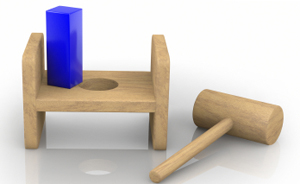
\includegraphics[width = 4in]{./images/squarePegRoundHole.jpg}
\end{figure}


./images/squarePegRoundHole.jpg\footnote{https://plus.maths.org/content/sites/plus.maths.org/files/puzzle/2012/hammer.jpg} is the location and name where the file must be stored to have it be inserted into the document.  Latex will scale the image to be 4 inches wide on the paper.  The images can be referred to by using the \ref{pegGame}.  The image number will be automatically populated and your text will point to the correct images, even if the image is located on a different page or if other images are put into the document before this image.  
 My favorite course is ECE \ref{pegGame}\ref{pegGame}\ref{pegGame}. 


\section*{Putting an * after section will remove the number from the section header.}

This document will have the following sections
\begin{enumerate}
\item  Document Text and Images
\item  Lists
\item  Math Mode
\item  Tables
\item  Style Sheet
\end{enumerate}

%paste the following line, without the comment character between \begin{document} and \maketitle
%\tableofcontents

\section{Math Mode}

There are quite a few special characters in \LaTeX that will cause errors if typed in normal text areas, such as dollar signs, percent signs, and ampersands.  These characters have special uses, but can be typed if they are preceded by the backslash escape character, such as \$, \%, and \&.  \% is used to comment text.  \$ is used to enter math mode, discussed in this section, and \& is used in tables, part of the next section.

Math mode is entered and exited by having a \$ in your document, without a backslash before the sign.  This makes it possible to enter mathamatical equations very quickly.  Subscripts are shown with undersscores.  There are $10_2$ types of people in the world, those that undestand binary and those that don't.  Superscripts are shown with the \^ symbol:  $10^2 = 100$.  Finally fractions are shown by using the frac command:  $\frac{1}{2} + \frac{1}{4} = \frac{3}{4}$

Use math mode to write out the Pythagorean theorem or the quadratic equation.

Here's a website with more details about math mode commands in Latex.

\url{https://en.wikibooks.org/wiki/LaTeX/Mathematics}

\section{Tables}

Here's an example of a table, the ``crl'' in the next line control the alignment of text within each column.  c = centered, r = right, and l = left.  Change the next line so that each column is centered. Modify this table to show something interesting to you.  If you have no interests, then use it to show the scores from the 2015-2016 OSU Football season.
\[ \begin{array}{crl}
\mbox{Number System}    & Decimal   & Binary    \\
\mbox{Zero}	            & 0         & 0         \\
\mbox{One} 	            & 1         & 1         \\
\mbox{Two} 	            & 2         & 10        \\
\mbox{Three}            & 3         & 11  	    \\
\mbox{Four}             & 4         & 100 	    \\
\mbox{Five}             & 5         & 101 	    \\
\mbox{Six}              & 6         & 110 	    \\
\mbox{Seven}            & 7         & 111 	    \\
\mbox{Eight}            & 8         & 1000 	    \\
\mbox{Nine}             & 9         & 1001 	    \\
\mbox{Ten} 	            & 10        & 1010 
\end{array}\] 

\newpage
\section{Style Sheet}
Open up the ECE111Notes.sty style sheet and change the following line from \newline
colorlinks=false,  \newline
to\newline
colorlinks=true\newline

Also, change the author field in the hypersetup area to be your name, the creator to be the name of the application used to type the .tex file, and the producer the name of the version of latex used to create the pdf, probably pdfLaTeX.

\centerimage{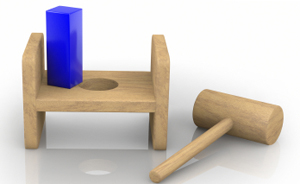
\includegraphics[width = 2in]{./images/squarePegRoundHole.jpg} }{This centerImage command is defined in ECE111Notes.sty.}{smallerPegGame} 

\vspace{2 in}
Submit the output pdf document to Canvas once you've finished this tutorial.

\end{document}
